\chapter{Literature Review}
\label{c:literature}

\section{Citations and Images} % 第二層標題,再更下一層的標題用\subsection{}
In this part of tutorial you will learn how to include images and cite the papers into your thesis. The default style of reference in this template is APA. If you want to change it to other styles, please head to line 25 of the thesis.tex file, follow the instructions then come back here.
To cite something, generate the BibTeX code from google scholar and paste it to the `bibliography.bib' file (\autoref{i:bib1} \& \autoref{i:bib2}). Since Google does not offer the doi, you have to add a comma after the second \{\} from the end and add doi=\{\} after it.

%引入圖片 (先將圖片上傳至figures資料夾再引用)

\begin{figure}[!htbp]
\centering %讓圖片水平置中
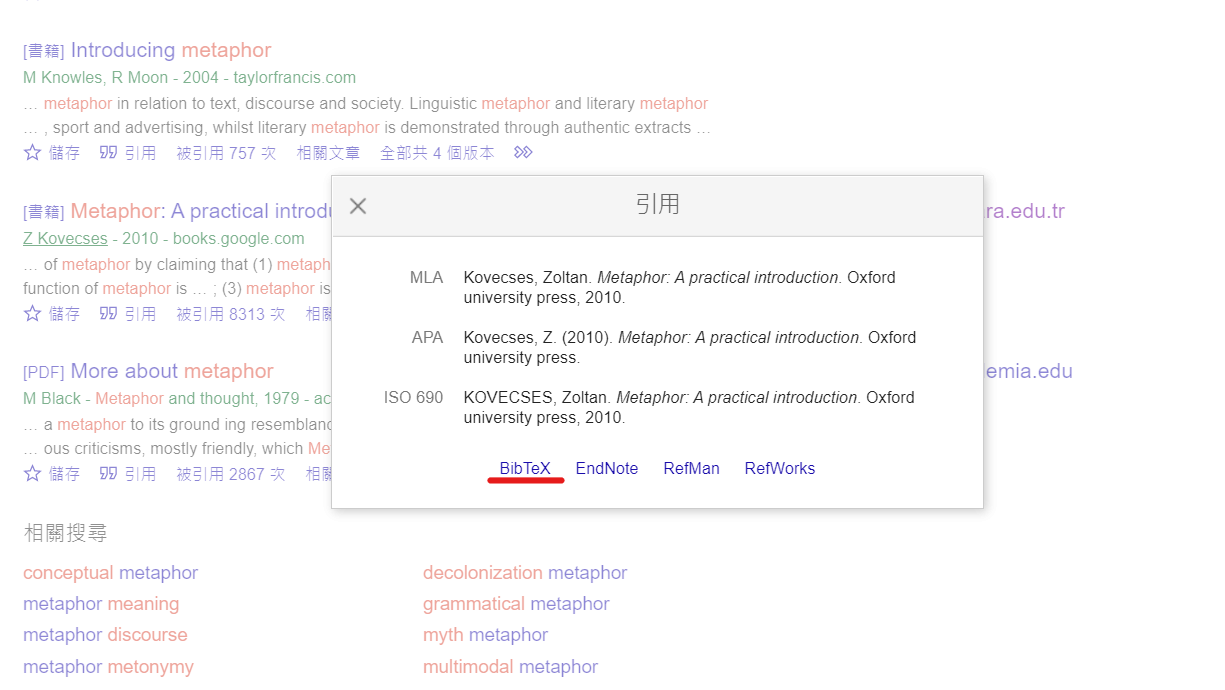
\includegraphics[width=1\textwidth]{figures/bib1.png}
% 1\textwidth 代表的是讓圖片剛好填滿設定的寬度,1就是100%的意思。所以如果想要他占80%就改成0.8
% 大括號裡面放的是圖片的位置,記得要加上副檔名
\caption{The way to generate BibTeX code in Google Scholar} %圖片的說明文字
\label{i:bib1} %圖片的標籤,在文內想提到這張圖片的時候會需要用到
\end{figure}

\begin{figure}[!htbp]
\centering %讓圖片水平置中
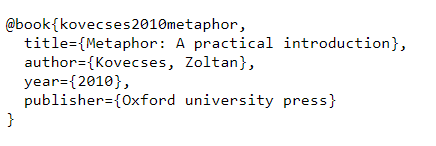
\includegraphics[width=1\textwidth]{figures/bib2.png}
\caption{The BibTeX code generated by Google Scholar} %圖片的說明文字
\label{i:bib2}
\end{figure}


% in-text citation
Then you can come back to this file and cite you reference like this:\par

\textcite{lin2014light} % author (year) 
did a study on the light verbs in Mandarin Chinese. \par
Conceptual metaphor is what is embodied in our conceptual systems (\cite{lakoff1980conceptual}). \par % author, year
\citeauthor{lin2014light}'s study provided some characteristics of the light verbs in Mandarin Chinese. \par % author name
A study of light verbs in Mandarin Chinese was done in \citeyear{lin2014light}. \par % year only
Some research have provided analysis on light verbs in Mandarin Chinese (\cite[e.g.,][]{lin2014light}). % to illustrate citations

% 大括號裡面一律放的是BibTeX code 裡的第一行,也就是他的標籤
% 如果是用中文撰寫的人,在引用時會建議先把google生成的標籤改成英文和數字的組合,以避免出現問題
% 有時候作者的名字裡面可能會出現重音或是點點,關於怎麼正確標示重音,請移步到bibliography.bib的第54行跟第66行
% bibliography 在生成的時候常常會遇到title大小寫未成功轉換的問題,請到bibliography.bib的第31行確認如何修改
% 你可以把滑鼠移到旁邊pdf的citation上面,會發現系統已經幫你做好跟reference的連結,而且也自動生成reference的頁面了。
% 如果要自行製作.bib檔,要視資料的性質標明其開頭,如書籍類是@book 來開頭,期刊文章使用@article 來起頭,例子如下:
% @article{ Knuth,
% author = "Knuth, Donald E.",
% year = "2004",
% title = "The {\TeX} Journal",
% journal = "SayYa-Publisher",
% volumn = " ",
% number = " ",
% pages = " ",
% month = " ",
% note = " ",}

% 每行後的逗點是必要的,名字的話Knuth, Donald E. 或Donald E. Knuth 這兩種方式,bibtex 都能認得,但姓擺在前面的時候其後要加個逗點,如果是兩位以上的作者時要以and來連接

% 另外,一些常見的書目管理也可以製作.bib檔,包含JabRef, BibDesk, Mendeley, Zotero 等。以JabRef為例,若要文獻的.bib格式可以在ads搜尋後 點擊文章  ,在Abstract下方會有Bibtex entry for this abstract的連結,點擊及可見到這篇文章的bib格式可直接複製貼上至bibliography.bib

\section{An Example paragraph}
With the outbreak of COVID-19, linguists have done research about it (\cite{mahlberg2021language,dong2021discourse,mcglashan2021networked}). For example, \textcite{hyland2021covid} investigated the hyperbolic and promotional language used in researchers' work on COVID-19. Posts on blogs about the pandemic were analysed, too (\cite{curry2021stance}). \textcite{curry2021stance} found that Spanish academic and English academic tend to use different stance nouns when it comes to COVID-related posts. Moreover, \citeauthor{muller2021communicating}'s research revealed distinct ways to mark uncertainty exist in British and German news (\citeyear{muller2021communicating}).\footnote{This is where your footnote goes.}
% 如果需要加註腳,直接再想加註腳的句子後面加上\footnote{}並將註腳內容打在大括號內
